\chapter{\glsentrylongsp{ci}}
\label{ch:sota-ci}

El comportamiento de una persona se ve influenciado por una gran cantidad de variables. Identificar las relaciones entre éstas es en la mayoría de las ocasiones una tarea que va de lo muy difícil a lo imposible, más aún si añadimos que éstas son muy numerosas y pueden llegar a ser imposibles de cuantificar o incluso de detectar.

La \ac{ci} engloba un conjunto de técnicas que facilitan enormemente estas tareas. En este capítulo se ofrece una perspectiva de la literatura actual sobre las técnicas de la inteligencia computacional que son de interés para esta tesis.

\section{\glsentrylongsp{ai} vs. \glsentrylongsp{ci}}

¿Qué es la \ac{ci}? Para entender el significado de éste término tenemos que entender cómo ha evolucionado el término \ac{ai} a lo largo de los años.

El primer concepto a introducir es el de "conexionismo". Se puede considerar a Santiago Ramón y Cajal como el principal precursor de esta idea por sus trabajos acerca de la estructura de las neuronas y su conexión (e.g. \cite{y1888estructura} y~\cite{ramon1904textura}). Otros prefieren citar el trabajo de Donald Hebb acerca de la Teoría del aprendizaje~\cite{hebb19680} como el primer trabajo sobre este tema. Independientemente, en el conexionismo se considera que la mente y el conocimiento surgen surgen de redes formadas por unidades sencillas interconectadas (e.g. neuronas).

Por otro lado, en 1950, Alan Turing publicó un artículo que comenzaba con la frase \textit{\enquote{Can machines think?\sidenote{Es aquí donde introduce el Test de Turing como método para probar si una máquina es capaz de exhibir un comportamiento inteligente similar al de un ser humano. El funcionamiento es el siguiente: hay tres participantes, dos humanos y una máquina, todos separados entre sí pero pudiendo intercambiarse mensajes de texto. Uno de los humanos le hace preguntas al otro humano y a la máquina, y éstos le responden. Si el humano que hace las preguntas no es capaz de discernir qué respuestas vienen de la máquina y qué respuestas del otro humano se puede concluir que la máquina es inteligente.}}}~\cite{turing1950computing}. Se puede considerar este momento como el punto donde se estableció el objetivo a largo plazo del campo de la \ac{ai}, ya que en el artículo Turing propuso un método para determinar si una máquina era capaz de pensar o no. Sin embargo, no fue hasta $1956$ en la Conferencia de Dartmouth~\cite{mccarthy1956dartmouth} donde John McCarthy acuñó el término~\ac{ai} a la vez que presentó el tema de la conferencia: "¿puede una máquina pensar\sidenote{Hay que destacar que el propio concepto de \enquote{pensar} es en sí un tema controvertido en el propio ser humano: ¿pensar es algo inherentemente biológico? ¿surje de la mente? Tanto si sí como si no, ¿de qué forma lo hace?. El experimento mental de la habitación china (ver~\cite{preston2002views}) propuesto por John Searle nace precisamente para rebatir la validez del Test de Turing. En esencia trata de un Test de Turing donde la máquina ha aprendido a hablar chino y es reemplazada por una persona que no sabe nada del idioma pero que va equipada con un listado de correspondencias del tipo "cada vez que entra esta secuencia de ideogramas, devuelve esta secuencia de ideogramas". Cuando una persona le manda mensajes en chino, esta otra responde, pero ¿podemos decir que dicha persona sabe chino? Evidentemente no. Entonces, cómo podemos asegurar que la máquina ha \enquote{aprendido} chino. Y lo que es más intrigante, si la máquina es capaz de realizar una acción sin entender lo que hace y por qué lo hace, ¿qué garantías tenemos de que el humano sí es capaz? Si los ordenadores operan sobre símbolos sin comprender el verdadero contenido de éstos, ¿hasta qué punto los humanos lo hacen de forma diferente}?".

En este punto la investigación en~\ac{ai} recibió muchísima atención por parte de investigadores y gobiernos, lo que se tradujo en financiación. Los estudios estaban dominados por aquellos relacionados con la idea del conexionismo hasta que aproximadamente en $1969$ se publicó el libro \textit{Perceptrons}~\cite{minsky1969perceptrons} de Marvin Minsky y Seymour Papert donde se expusieron las limitaciones de los modelos de redes neuronales desarrollados hasta la fecha. El impacto fue tal que se abandonó prácticamente por completo el campo de conexionismo, y por tanto una gran parte de la investigación en la \ac{ai}. Es lo que se conoce como \textit{AI Winter}\footnote{Indicar que también hubo otros factores como los ecnómicos, la crisis del software, etcétera. https://en.wikipedia.org/wiki/AI\_winter\#Lasting\_effects\_of\_the\_AI\_winters}.

Debido al \textit{AI Winter}, el conexionismo no estuvo presente en la literatura científica durante prácticamente dos décadas. Fue en $1980$ cuando apareció un nuevo concepto dentro de la \ac{ai} que acaparó el interés por el campo de nuevo y que se considera como el primer caso de éxisto dentro del campo: los Sistemas Expertos~\cite{russell2003artificial}. A finales de la década, sin embargo, empezaron a resurgir los enfoques conexionistas, en gran parte por el surgimiento de nuevas formas de entrenamiento de redes multicapa o por el concepto de funciones de activación no lineales (e.g. trabajos como~\cite{rumelhart1985learning} o~\cite{cybenko1989approximation}). En este momento los sistemas expertos empezaron a perder interés\footnote{A esta década se la conoce como segundo \textit{AI Winter} dado que la investigación sobre Sistemas Expertos se empieza a abandonar. Sin embargo no fue un abandono tan acusado como el del primer AI Winter.} frente al nuevo avance del conexionismo.

Frente al avance del conexionismo, algunas voces se alzaron contra lo que se consideraba como \enquote{el enfoque incorrecto} de la \ac{ai}\footnote{Es comprensible ya que el método clásico produce modelos fáciles de interpretar mientras que el enfoque conexionista produce modelos cuyo funcionamiento en general no es del todo deducible.}. Mientras que el enfoque clásico de la \ac{ai} postulaba que la mente operaba de la misma manera que una máquina de Turing, es decir, mediante operaciones sobre un lenguaje de símbolos, el enfoque del conexionismo postulaba que la mente, el comportamiento inteligente emergía de modelos a más bajo nivel. Además, otras técnicas no pertenecientes al conexionismo pero sí alienadas a éste debido a su enfoque de comportamiento emergente y aproximación (e.g. lógica difusa o algoritmos genéticos) ganaban popularidad y alimentaban el éxito de este tipo de técnicas que no cumplian el ideal de la aproximación exacta y simbólica de la \ac{ai}.

Esto provocó una explosión de terminologías para diferenciar las investigaciones de la propia~\ref{ai} clásica. Por un lado, se evitaba el conflicto nombrando el trabajo con un término más acorde con el comportamiento o técnica utilizada. Por otro, se separaba de las connotaciones negativas de \enquote{promesas incumplidas} que el término había adquirido con el paso de los años.

\begin{figure}
	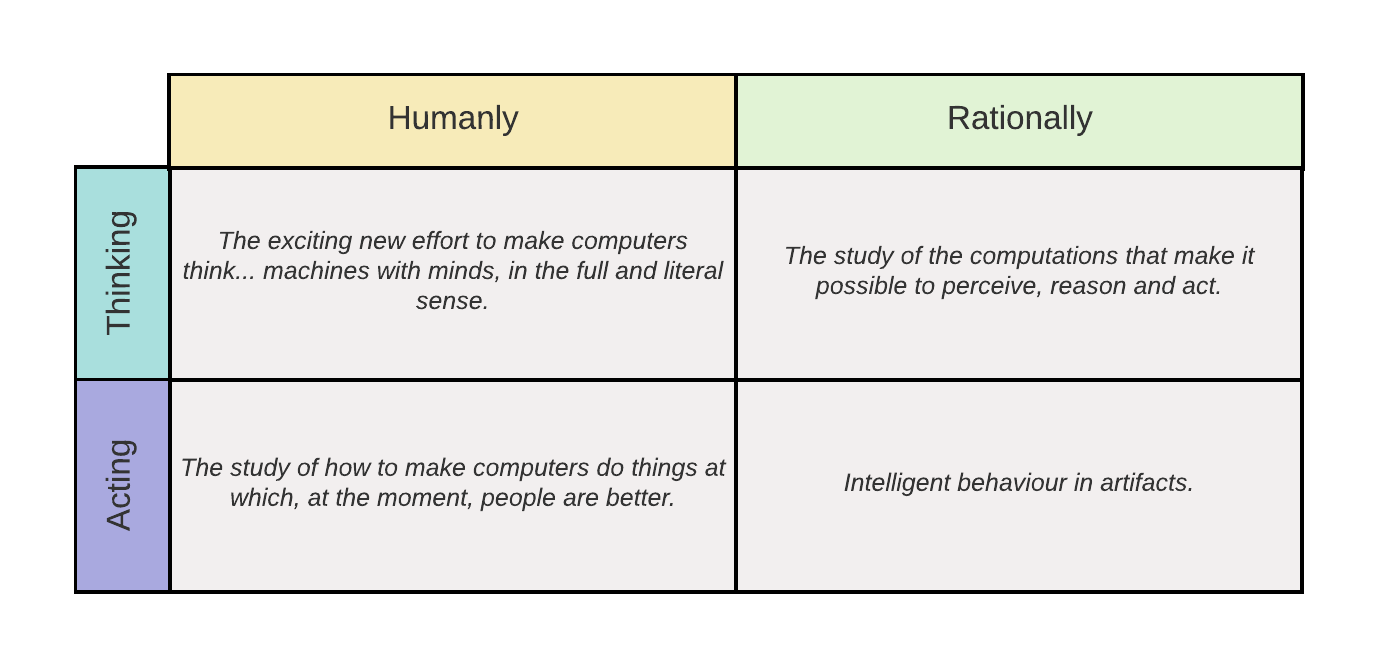
\includegraphics{different-povs-ai}
	\caption{Objetivos que persigue la~\glsentrylong{ai}. Las filas diferencian si lo que se persigue es pensamiento o comportamiento mientras que las columnas separan si se persigue la inteligencia entendida como la humana o como el ideal de inteligencia (inteligencia racional).}
	\label{fig:different-povs-ai}
\end{figure}

Lo verdaderamente interesante es ver la evolución de la literatura, y por tanto de los objetivos de la \ac{ai} durante estos años. En el nacimiento del campo, se buscan literalmente máquinas que piensen como humanos, aunque en el conexionismo se habla de algo más general como lo es la mente. Con el paso de los años y los continuos choques con la realidad, la literatura gira hacia la búsqueda de conductas y comportamientos inteligentes, sin necesidad de que cubran todos los aspectos que hacen de un ser un ente inteligente. Es más, en el momento en que la cantidad de diferente terminología empieza a elevarse, se pone de manifiesto que existen diferentes puntos de vista para el mismo campo. En~\cite{russell2003artificial}, tras un análisis de las definiciones existentes en la literatura por parte de diferentes autores, se hace énfasis en este hecho mostrando los diferentes puntos de vista a la hora de hablar de lo que es la \ac{ai} (estos son sistemas que piensan como humanos, que actúan como humanos, que piensan racionalmente y que actúan racionalmente).

Volviendo al tema de la terminología, muchas de las diferentes técnicas se fueron agrupando dentro de diferentes áreas. Una de ellas es la conocida como \glsentrylong{ci}. Dado que persigue el mismo objetivo a largo plazo y que surje de la propia \ac{ai} parece lógico mantenerla como un subconjunto y no como un nuevo campo del conocimiento humano. La principal diferencia es la generalización de esa disputa o diferentes puntos de vista, la \ac{ai} clásica y los métodos no clásicos.

Podemos definir la \ac{ci} como la rama de la \ac{ai} que explora la búsqueda de conocimiento a partir del aprendizaje a partir de datos experimentales. A diferencia de la aproximación clásica de la \ac{ai}, buscan aproximaciones a la soluciones y no las soluciones exactas \textit{per se}. Esto es debido de la necesidad de otros puntos de vista en resolución de problemas cuando éstos son muy complejos, cuando los datos están incompletos o contienen ruido o cuando no pueden ser traducidos al lenguaje binario.

Se puede fijar el año $1994$ como el que el término \ac{ci} nace como área, coincidiendo con el cambio de nombre del \textit{IEEE Neural Networks Council} a \textit{IEEE Computational Intelligence Society}\footnote{\url{http://cis.ieee.org/}.}. Poco antes, en $1993$, Bob Marks en su trabajo~\cite{bezdek1993intelligence} presentó las que él consideraba diferencias fundamentales entre la \ac{ai} y la \ac{ci} para posteriormente resumirlas en la siguiente frase.

\blockquote{"Neural networks, genetic algorithms, fuzzy systems, evolutionary programming, and artificial life are the building blocks of CI.}

Durante estos años ganaba popularidad el concepto del \ac{sc}. Éste engloba las técnicas que buscan resolver problemas que manejan información incompleta o con ruido. Debido a que el conjunto de técnicas definidas como consituyentes del \ac{sc} son las mismas que las de la \ac{ci} algunos autores consideran el \ac{sc} como la rama que ocupa estas técnicas mientras que otros consideran ambos términos equivalentes. Nosotros consideramos que el \ac{sc} es un punto de vista de la computación más que de la \ac{ai} en contraposición con el \ac{hc}, y que la \ac{ci} hace uso de métodos del \ac{sc}.

\TODO Aquí dibujo de una taxonomía donde así: (inteligencia (clásica (hard computing)) (computacional (soft computing (lógica difusa, computación evolutiva, redes neuronales))))

"AI ranges from machines truly capable of thinking to search algorithms used to play board games"
"It has applications in nearly every way we use computers in society."
"The term artificial intelligence was first coined by John McCarthy in 1956 when he held the first academic conference on the subject"
"¿Puede una máquina pensar?. 
"Is the problem simply that we haven’t focused
enough resources on basic research, as is seen in the AI winter section, or is the complexity of AI one that we
haven’t yet come to grasp yet? (And instead, like in the case of computer Chess, we focus on much more
specialized problems rather than understanding the notion of ‘understanding’ in a problem domain.)"

Inteligencia computacional: habilidad de un ordenador de aprender una tarea específica a partir de datos u observaciones experimentales (esto es sacado de la wikipedia. Hay que buscar más definiciones en la literatura). Destacar \textbf{tarea específica} y \textbf{a partir de datos experimentales}.

Algunos autores lo consideran sinónimo de Soft Computing, pero no como no hay definición comúnmente aceptada, pues na.

La cosa es que hay procesos matemáticos muy complejos, con mucha interdependencia entre variables y factores que hacen que los problemas sean muy difíciles de modelar, más aún cuando el problema en su naturaleza es estocástico (poner algún ejemplo de algo en la naturaleza que se comporte de forma estocástica~\cite{siddique2013computational}).

But generally, computational intelligence is a set of nature-inspired computational methodologies and approaches to address complex real-world problems to which mathematical or traditional modelling can be useless for a few reasons: the processes might be too complex for mathematical reasoning, it might contain some uncertainties during the process, or the process might simply be stochastic in nature.[1] Indeed, many real-life problems cannot be translated into binary language (unique values of 0 and 1) for computers to process it. Computational Intelligence therefore provides solutions for such problems.



\section{Inteligencia computacional}

Qué es la inteligencia artificial. Qué es la inteligencia computacional.
Diferencias entre inteligencia artificial clásica e inteligencia computacional. Diferentes puntos de vista (soft computing, machine learning, ...)
Técnicas de entrenamiento de modelos: supervisado, no supervisado, semisupervisado, refuerzo, ...
Técnias de funcionamiendo: online y offline
Técnicas de la inteligencia computacional usadas en esta tesis (redes neuronales artificiales(perceptrón multicapa, recurrentes y lstm), lógica difusa y computación evolutiva)
¿Qué técnicas se usan actualmente y sobre qué problemas?
Detección de patrones de eficiencia y agresividad de subyacen en los comportamientos de éstosç
Estudio de la efectividad de los sistemas de asistencia para mejorar la eficiencia de conducción
Estudio de los sistemas de asistencia para analizar el comportamiento del conductor.